\chapter{The way of the program}

The goal of this book is to teach you to think like a computer scientist. This
way of thinking combines some of the best features of mathematics,
engineering, and natural science. Like mathematicians, computer scientists use
formal languages to denote ideas (specifically computations). Like engineers,
they design things, assembling components into systems and evaluating
tradeoffs among alternatives. Like scientists, they observe the behavior of
complex systems, form hypotheses, and test predictions. \index{problem
solving}

The single most important skill for a computer scientist is {\bf problem
solving}. Problem solving means the ability to formulate problems, think
creatively about solutions, and express a solution clearly and accurately. As
it turns out, the process of learning to program is an excellent opportunity
to practice problem-solving skills. That's why this chapter is called, ``The
way of the program''.

On one level, you will be learning to program, a useful skill by itself. On
another level, you will use programming as a means to an end. As we go along,
that end will become clearer.


\section{What is a program?}

A {\bf program} is a sequence of instructions that specifies how to perform a
computation. The computation might be something mathematical, such as solving
a system of equations or finding the roots of a polynomial, but it can also be
a symbolic computation, such as searching and replacing text in a document or
something graphical, like processing an image or playing a video.
\index{program}

The details look different in different languages, but a few basic
instructions appear in just about every language:

\begin{description}

\item[input:] Get data from the keyboard, a file, the network,  a camera, or
some other device like a fingerprint reader.

\item[output:] Display data on the screen, save it in a file, send it over the
network, or control a device such as a door lock.

\item[math:] Perform basic mathematical operations like addition and
multiplication.

\item[decisions:] Check for certain conditions to determine whether to perform
some action. For example: if the fingerprint matches, unlock the door.

\item[repetition:] Perform some action repeatedly, usually with some
variation.

\end{description}

Believe it or not, that's pretty much all there is to it. Every program you've
ever used, no matter how complicated, is made up of instructions that look
pretty much like these. So you can think of programming as the process of
breaking a large, complex task into smaller and smaller subtasks until the
subtasks are simple enough to be performed with one of these basic
instructions.


\section{Running Go}
\index{Go!running}

One of the challenges of getting started with Go is that you might have to
install Go and related software on your computer. If you are familiar with
your operating system, and especially if you are comfortable with the command-
line interface, you will have no trouble installing Go. But for beginners, it
can be distracting to learn about system administration and programming at the
same time.

To avoid that problem, we recommend that you start out using the
{\it Go Playground}:
\index{Go Playground}

\url{https://play.golang.org/}

The {\it Go Playground} lets you type or paste Go code and click a button
to run it, without installing anything. It is limited in many ways, but good
enough to get started. After you've taken the first steps, we'll provide
instructions for installing Go on your computer.\footnote{If you can't wait to
install Go, Appendix A explains how.}


\section{The hello world program}
\label{hello}

Traditionally, the first program you write when learning a new programming
language is called the hello world program. All it does is display the
words ``Hello, World!''\ on the screen.
In Go, it looks like this:

\index{hello.go}
\lstinputlisting[language=Golang,label=lst:hello.go]{01/hello/hello.go}

We typed listing \ref{lst:hello.go} and saved it in the playground.
Follow this link to see it:

\url{https://tgo.li/2r8yCXj}

If you open that address in a browser, you'll see a page similar to Figure~\ref{fig:playhello}.

\begin{figure}[!ht]
\begin{center}
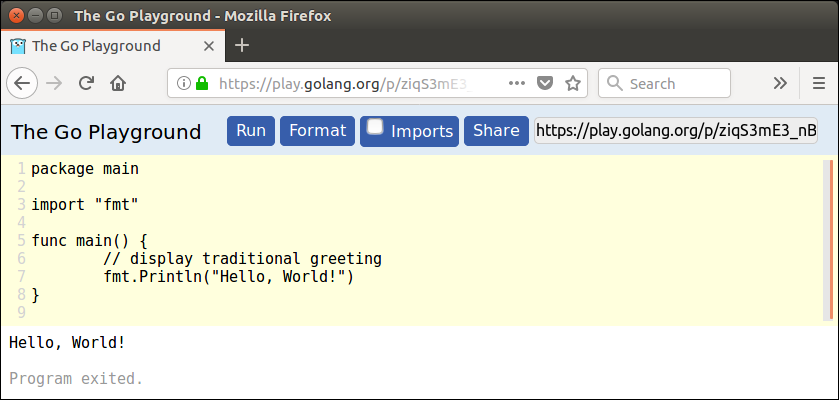
\includegraphics[width=1.0\textwidth]{figs/play-hello.png}
\caption{The hello world program in the Go playground (after running).}
\label{fig:playhello}
\end{center}
\end{figure}

To execute the program, click the blue button labeled {\bf Run}. You may
briefly see the message {\tt Waiting for remote server...}, and then the
output will appear below the code listing, as pictured. Note that the output
does not include the quotation marks around ``Hello, World!''\ .

We want invite you to try editing the hello world program, but we need words
to describe parts of a program so we can talk about it. The next section
covers some basic terms.


\section{Program structure}
\label{program structure}

Go programs are made up of {\bf declarations}. In listing \ref{lst:hello.go}
we have three declarations: {\tt package}, {\tt import}, and {\tt func}.

We'll have a lot more to say about those declarations, but basically this is
what they mean, starting with the most fundamental one, {\tt func}:

\begin{description}

\item[\textbf{\texttt{func}}:] This declares a {\bf function}, which is a
sequence of lines of code that perform some computation or action. The only
function in \ref{lst:hello.go} is named {\tt main}.

\item[\textbf{\texttt{package}}:] All Go code is organized in {\bf packages},
which consist of one or more {\tt .go} files. The package name {\tt main} is
mandatory for stand-alone programs --- as opposed to {\bf library packages}
that are not complete programs, but provide functions for other programs.

\item[\textbf{\texttt{import}}:] This declaration tells Go which library
packages are needed to build our program. Our {\tt main} function uses the
{\tt fmt.Println} function, therefore we need to import {\tt fmt}. The
{\tt fmt} package provides text formatting and output functions.

\end{description}

Programming in Go is writing functions in {\tt .go} files that belong
packages. Usually our functions will use functions from library packages
that we import. In this book we'll mostly write stand-alone programs, but
we'll use many libraries written by others.


\section{Exercises}

\begin{exercise}

It is a good idea to read this book in front of a computer so you can try out
the examples as you go. In this exercise, we'll use the {\it Go Playground}
to learn about the structure of the {\tt hello.go} program.

Whenever you are experimenting with a new feature, you should try to make
mistakes. 

This kind of experiment helps you remember what you read; it also
helps when you are programming, because you get to know what the error
messages mean. It is better to make mistakes now and on purpose than
later and accidentally.
\index{error message}

Start with {\tt hello.go} in the {\it Go Playground} and make the changes
suggested here. To recover the original code, just visit that same URL:

\url{https://tgo.li/2r8yCXj}

After each change, hit the {\bf Run} button to see what happens.

\begin{enumerate}

\item What happens when there is no {\tt package} declaration?

\item What if the {\tt package} name is {\tt banana} instead of {\tt main}? 

\item Restore the program to its original state. Then remove all blank lines
and the whitespace to the left of {\tt fmt.Println("Hello, World!")}. Does the
program still run? What happens when you click the {\bf Format} button?

\item What happens when there is no {\tt import} declaration? After trying 
to run the program without the {\tt import} line, check the box labeled
{\bf Imports}, then click {\bf Format} and note what happens.

\item There is only one line with text in {\tt hello.go} that you can delete
without changing the behavior of the program. Can you discover which one?
Can you guess its purpose, since it does not affect the program?


\end{enumerate}

\end{exercise}


\section{Anatomy of a function}
\label{function!syntax}

Let's take a closer look at the {\tt main} function from \ref{lst:hello.go}:

\begin{lstlisting}
func main() {
	// display traditional greeting
	fmt.Println("Hello, World!")
}
\end{lstlisting}

\index{main}

The {\tt func} keyword is followed by the function name. A program can have
many functions, so we try to give descriptive names to them. The name {\tt
main} is not very descriptive, but is special: the execution of a Go program
begins and ends in the function called {\tt main}. Everything else that
happens when the program runs depends on actions started by {\tt main}.

\index{\{\} curly braces}
\index{brackets!curly}

Every function has a body: a sequence of lines delimited by curly braces
({\tt\{} and {\tt\}}). The content of the body is indented from the left
margin to make it clear where it starts and ends. In Go, the opening brace is
always at the first line of a declaration that has a body. For example, this
is wrong:

\begin{lstlisting}
func main()
{
	// WRONG: the { should be in the top line of the declaration
	fmt.Println("Hello, World!")
}
\end{lstlisting}

\index{comment!end-of-line}
\index{statement!comment}

Any line that begins with two slashes {\tt //} is a {\bf comment}: English
text that explains the code. When Go sees {\tt //}, it ignores everything from
there until the end of the line. Comments have no effect on the execution of
the program, but they make it easier for other programmers (and your future
self) to understand what you meant to do.

The second line in the body of {\tt main} main is a {\bf statement}, a line of
code that performs a basic action. A common way of performing actions is to
call functions from library packages. In the hello world program, this
statement calls the {\tt fmt.Println} function to display a message on the
screen:

\begin{lstlisting}
	fmt.Println("Hello, World!")
\end{lstlisting}

The name {\tt Println} stands for ``print line''. Confusingly, in programming,
{\em print} can mean both ``display on the screen'' and ``send to the
printer''. In this book, we'll try to say ``display'' when we mean output to
the screen.

\index{case-sensitive}
Go is ``case-sensitive'', which means that uppercase
and lowercase are not the same. In this example, {\tt Println} has to begin
with an uppercase letter; {\tt println} and {\tt PRINTLN} won't work.

\section{Exercises}

\begin{exercise}

Once again, start with {\tt hello.go} in the {\it Go Playground} and make the
changes suggested here. To recover the original code, just visit that same
URL:

\url{https://tgo.li/2r8yCXj}

After each change, hit the {\bf Run} button to see what happens. Pay attention
to the error messages.

\begin{enumerate}

\item Change the text of the function call {\tt fmt.Println("Hello, World!")}
to make it invalid by removing parenthesis.

\item If you are trying to print a string, what happens if you leave out one
of the quotation marks, or both?

\item Add another call to {\tt fmt.Println("")} below the first one, putting
your own text between the quotes.


\end{enumerate}

\end{exercise}



\section{Formal and natural languages}
\index{formal language}
\index{natural language}
\index{language!formal}
\index{language!natural}

{\bf Natural languages} are the languages people speak, such as English,
Spanish, and French. They were not designed by people (although people try to
impose some order on them); they evolved naturally.

{\bf Formal languages} are languages that are designed by people for specific
applications. For example, the notation that mathematicians use is a formal
language that is particularly good at denoting relationships among numbers and
symbols. Chemists use a formal language to represent the chemical structure of
molecules. And most importantly:

\begin{quote}
{\bf Programming languages are formal languages that have been
designed to express computations.}
\end{quote}

Formal languages tend to have strict {\bf syntax} rules that govern the
structure of statements. For example, in mathematics the statement $3 + 3 = 6$
has correct syntax, but $3 + = 3 \$ 6$ does not. In chemistry $H_2O$ is a
syntactically correct formula, but $_2Zz$ is not.
\index{syntax}

Syntax rules come in two flavors, pertaining to {\bf tokens} and structure.
Tokens are the basic elements of the language, such as words, numbers, and
chemical elements. One of the problems with $3 += 3 \$ 6$ is that \( \$ \) is
not a legal token in mathematics (at least as far as we know). Similarly,
$_2Zz$ is not legal because there is no element with the abbreviation $Zz$.
\index{token}
\index{structure}

The second type of syntax rule pertains to the way tokens are
combined. The equation $3 += 3$ is illegal because even though $+$
and $=$ are legal tokens, you can't have one right after the other.
Similarly, in a chemical formula the subscript comes after the element
name, not before.

This is @ well-structured Engli\$h sentence with invalid t*kens in it. This
sentence all valid tokens has, but invalid structure with.

When you read a sentence in English or a statement in a formal language, you
have to figure out the structure (although in a natural language you do this
subconsciously). This process is called {\bf parsing}. \index{parse}

Although formal and natural languages have many features in common---tokens,
structure, and syntax---there are some differences:
\index{ambiguity}
\index{redundancy}
\index{literalness}

\begin{description}

\item[ambiguity:] Natural languages are full of ambiguity, which
people deal with by using contextual clues and other information.
Formal languages are designed to be nearly or completely unambiguous,
which means that any statement has exactly one meaning,
regardless of context.

\item[redundancy:] In order to make up for ambiguity and reduce
misunderstandings, natural languages employ lots of redundancy. As a result,
they are often verbose. Formal languages are less redundant and more concise.

\item[literalness:] Natural languages are full of idiom and metaphor. If we
say, ``The penny dropped'', there is probably no penny and nothing dropping
(this idiom means that someone understood something after a period of
confusion). Formal languages mean exactly what they say.

\end{description}

Because we all grow up speaking natural languages, it is sometimes hard to
adjust to formal languages. The difference between formal and natural language
is like the difference between poetry and prose, but more so: \index{poetry}
\index{prose}

\begin{description}

\item[Poetry:] Words are used for their sounds as well as for their meaning,
and the whole poem together creates an effect or emotional response. Ambiguity
is not only common but often deliberate.

\item[Prose:] The literal meaning of words is more important, and the
structure contributes more meaning. Prose is more amenable to analysis than
poetry but still often ambiguous.

\item[Programs:] The meaning of a computer program is unambiguous and literal,
and can be understood entirely by analysis of the tokens and structure.

\end{description}

Formal languages are more dense than natural languages, so it takes longer to
read them. Also, the structure is important, so it is not always best to read
from top to bottom, left to right. Instead, learn to parse the program in your
head, identifying the tokens and interpreting the structure. Finally, the
details matter. Small errors in spelling and punctuation, which you can get
away with in natural languages, can make a big difference in a formal
language.


\section{Running Go programs on your machine}

The {\it Go Playground} imposes several limitations for security and cost
reasons. For example, the program in listing \ref{lst:now.go} should tell
you the current time, but it will always claim it is 11 PM, November 10,
2009---the date when Go was announced to the public. 

\index{now.go}
\lstinputlisting[language=Golang,label=lst:now.go]{01/now/now.go}

The playground also automates and hides important concepts and actions, which
this section reveals.


\index{machine language}
\index{compile}
\index{source code}
\index{object code}
\index{executable}

Before they can run, programs written in Go must be translated into ``machine
language'', the low-level instructions that the computer can follow. This
translation is done by the Go {\bf compiler}, one of the software tools that
comes with the Go distribution.

The compiler reads {\tt .go} text files---the {\bf source code}---and produces
binary files that are executable. In this book we'll use two command-line Go
tools to run our programs:

\begin{description}

\item[\textbf{\texttt{go build}}:] This command reads the {\tt .go} files in
the current directory. If a {\tt package main} is found, the files are compiled
to produce an executable. You then use the OS shell to run the executable.

\item[\textbf{\texttt{go run }}{\tt myprogram.go}:] If the file {\tt myprogram.go}
declares a {\tt package main}, it is compiled to a temporary directory and
immediately executed.

\end{description}

The {\tt go build} command requires an extra step to run the program, but on
the other hand it gives you a stand-alone executable that does not depend
on having the Go tools installed, so it can easily be distributed.

\subsection{Using \tt{go run}}


\subsection{Using \tt{go build}}


When we run {\tt go build}  with the same name as the current directory
(an {\tt .exe} extension is added if you are on Windows)


Once a program is compiled, you can execute it repeatedly without further translation.
As a result, compiled programs often run faster than interpreted programs.

Figure~\ref{fig.compiler} shows the steps of the development process.

\begin{figure}[!ht]
\begin{center}
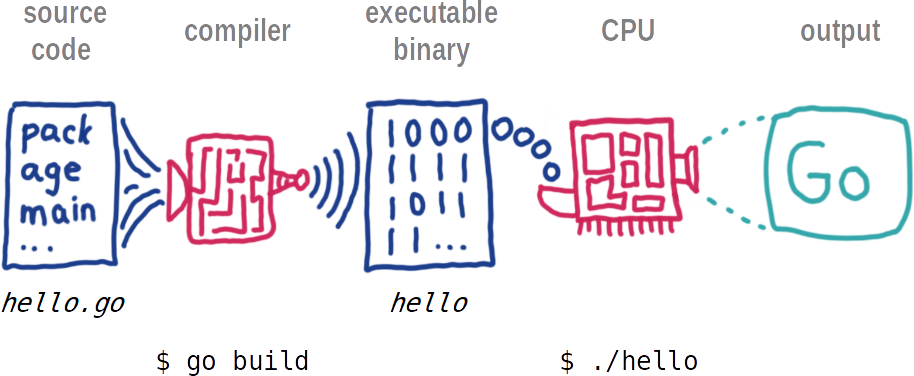
\includegraphics{figs/compiler.png}
\caption{The process of compiling and running a Go program.}
\label{fig.compiler}
\end{center}
\end{figure}

The Go playground (shown in Figure~\ref{fig.playhello}) lets us use a Go compiler running on a Google server machine.
When you hit the {\bf Run} button, the playground Go compiler produces an executable and saves it in the server (if there are no errors).
The server then runs the executable, and sends its output back to your browser.
The executable is then discarded, so the Go playground is useful only for quick experiments.

To compile Go programs locally, we need to install the Go distribution, as explained in Appendix XXX. After Go is installed, you can use the {\tt go build} in the terminal.

% LR: 2018-01-10: chose a tone: "you" or "the programmer" (see surrounding paragraphs)

The programmer writes source code in the file {\tt hello.go} and uses {\tt go build} to compile it.
If there are no errors, the compiler saves the executable in the file {\tt hello} (or {\tt hello.exe}, in Windows).
To run the program, the user simply invokes it in the terminal.
The output of the program is then displayed on the screen.

This is how running {\tt hello.go} looks like on the {\tt bash} shell installed by default on GNU/Linux and Mac OS X machines:

\begin{verbatim}
$ ./hello 
Hello, World!
\end{verbatim}

On the Windows command prompt, it's very similar:

\begin{verbatim}
> hello.exe 
Hello, World!
\end{verbatim}


Although it might seem complicated, these steps are automated for you in most program development environments.
Usually you only have to press a button or type a single command to compile and run your program.
On the other hand, it is important to know what steps are happening in the background,
so if something goes wrong you can figure out what it is.



\section{Debugging}
\index{debugging}

Programmers make mistakes. For whimsical reasons, programming errors are
called {\bf bugs} and the process of tracking them down is called {\bf
debugging}.
\index{debugging}
\index{bug}

Programming, and especially debugging, sometimes brings out strong emotions.
If you are struggling with a difficult bug, you might  feel angry, despondent,
or embarrassed.

There is evidence that people naturally respond to computers as if they were
people. When they work well, we think of them as teammates, and when they are
obstinate or rude, we respond to them the same way we respond to rude,
obstinate people (Reeves and Nass, {\it The Media  Equation: How People
Treat Computers, Television, and New Media Like Real People and Places}).
\index{debugging!emotional response}
\index{emotional debugging}

Preparing for these reactions might help you deal with them. One approach is
to think of the computer as an employee with certain strengths, like speed and
precision, and particular weaknesses, like lack of empathy and inability to
grasp the big picture.

Your job is to be a good manager: find ways to take advantage of the strengths
and mitigate the weaknesses. And find ways to use your emotions to engage with
the problem, without letting your reactions interfere with your ability to
work effectively.

Learning to debug can be frustrating, but it is a valuable skill that is
useful for many activities beyond programming. At the end of each chapter
there is a section, like this one, with my suggestions for debugging. we hope
they help!


\section{Glossary}

\begin{description}

\item[problem solving:]  The process of formulating a problem, finding
a solution, and expressing it.
\index{problem solving}

\item[declaration:] One of the main parts of a Go source code file, such
as {\tt import} or {\tt func} 
\index{declaration}

\item[high-level language:]  A programming language like Go that
is designed to be easy for humans to read and write.
\index{high-level language}

\item[low-level language:]  A programming language that is designed
to be easy for a computer to run; also called ``machine language'' or
``assembly language''.
\index{low-level language}

\item[portability:]  A property of a program that can run on more
than one kind of computer.
\index{portability}

\item[interpreter:]  A program that reads another program and executes
it
\index{interpret}

\item[prompt:] Characters displayed by the interpreter to indicate
that it is ready to take input from the user.
\index{prompt}

\item[program:] A set of instructions that specifies a computation.
\index{program}

\item[print statement:]  An instruction that causes the Python
interpreter to display a value on the screen.
\index{print statement}
\index{statement!print}

\item[operator:]  A special symbol that represents a simple computation like
addition, multiplication, or string concatenation.
\index{operator}

\item[value:]  One of the basic units of data, like a number or string, 
that a program manipulates.
\index{value}

\item[type:] A category of values. The types we have seen so far
are integers (type {\tt int}), floating-point numbers (type {\tt
float}), and strings (type {\tt str}).
\index{type}

\item[integer:] A type that represents whole numbers.
\index{integer}

\item[floating-point:] A type that represents numbers with fractional
parts.
\index{floating-point}

\item[string:] A type that represents sequences of characters.
\index{string}

\item[natural language:]  Any one of the languages that people speak that
evolved naturally.
\index{natural language}

\item[formal language:]  Any one of the languages that people have designed
for specific purposes, such as representing mathematical ideas or
computer programs; all programming languages are formal languages.
\index{formal language}

\item[token:]  One of the basic elements of the syntactic structure of
a program, analogous to a word in a natural language.
\index{token}

\item[syntax:] The rules that govern the structure of a program.
\index{syntax}

\item[parse:] To examine a program and analyze the syntactic structure.
\index{parse}

\item[bug:] An error in a program.
\index{bug}

\item[debugging:] The process of finding and correcting bugs.
\index{debugging}

\end{description}


\section{Exercises}

\begin{exercise}

It is a good idea to read this book in front of a computer so you can
try out the examples as you go.

Whenever you are experimenting with a new feature, you should try
to make mistakes. For example, in the ``Hello, world!'' program,
what happens if you leave out one of the quotation marks?  What
if you leave out both?  What if you spell {\tt print} wrong?
\index{error message}

This kind of experiment helps you remember what you read; it also
helps when you are programming, because you get to know what the error
messages mean. It is better to make mistakes now and on purpose than
later and accidentally.

\begin{enumerate}

\item In a print statement, what happens if you leave out one
of the parentheses, or both?

\item If you are trying to print a string, what happens if you
leave out one of the quotation marks, or both?

\item You can use a minus sign to make a negative number like
{\tt -2}. What happens if you put a plus sign before a number?
What about {\tt 2++2}?

\item In math notation, leading zeros are ok, as in {\tt 02}.
What happens if you try this in Python?

\item What happens if you have two values with no operator
between them?

\end{enumerate}

\end{exercise}



\begin{exercise}

Start the Python interpreter and use it as a calculator.

\begin{enumerate}

\item How many seconds are there in 42 minutes 42 seconds?

\item How many miles are there in 10 kilometers?  Hint: there are 1.61
  kilometers in a mile.

\item If you run a 10 kilometer race in 42 minutes 42 seconds, what is
  your average pace (time per mile in minutes and seconds)?  What is
  your average speed in miles per hour?

\index{calculator}
\index{running pace}

\end{enumerate}

\end{exercise}
